
  % Assignment 3
  \question Explain the reasoning behind the definition of the ideal throughput. Which sort of traffic scenarios is it best suited to?
  \begin{solution}
    First, we define ideal throughput. Let $G = (N, C)$ be a topology, where $N$ is a set of nodes and $C$ is a set of channels. To start we fix some particular routing $R = \{R_n\}_{n \in N}$, that is, for each $n \in N$, $R_n$ denotes a set of routes starting at $n$ (a route is a list of channels that defines a path). We further suppose all channels have bandwidth $b\;\si{\bit\per\second}$. We define the \emph{load} $\gamma_c$ on a particular channel $c$ to be the number of routes using channel $c$. Precisely,
    \[ \gamma_c = \left\lvert \left\{ r \in R_n: c \in r, n \in N \right\} \right\rvert. \]
    We define the \emph{maximum channel load}, $\gamma_\text{max}$ to be maximum load over all channels, that is
    \[ \gamma_\text{max} = \max_{c \in C} \{\gamma_c\}. \]
    A channel $c \in C$ such that $\gamma_c = \gamma_\text{max}$ is said to be a \emph{bottleneck channel}.
    We define the ideal throughput to be the number of bits that can be sent over a bottleneck channel in the scenario that every route that utilises that channel contests for it at the same time. Formally,
    \[ \theta_{\text{ideal}} = \frac{b}{\gamma_\text{max}}. \]
    Ideal throughput gives us the notion of the maximum size (in bits) of a message such that we can send it along a route in the worst case scenario without contest. It is optimal for traffic scenarios where $\gamma_\text{max} - \overline\gamma$ is small, where $\overline\gamma$ denotes the mean channel load for $C$. To illustrate why, consider a traffic scenario on a large network where all channels have bandwidth $\SI{1024}{\bit\per\second}$ with one channel $c'$ such that $\gamma_{c'} = 16$ and for all $c \in C \setminus \{c'\}$ we have $\gamma_c = 1$. Then, $\gamma_\text{max} = 16$, thus $\theta_\text{ideal} = \frac{1024}{16} = 64$. Thus, to ensure that we do not cause performance issues each message must have size $\SI{64}{\bit}$. As this is a large network, we see that this is causing lots of channels to have $\SI{960}{\bit}$s of bandwidth unused, and so our ideal throughput is not giving us a good picture in this scenario.
  \end{solution}

  \question Suppose that we have 260 processors, each with 60 pins and so that the signal frequency is $\SI{1}{\giga\hertz}$; moreover, the router delay of any router is $\SI{15}{\nano\second}$. Our intention is to design an interconnection network that is a hypercube, a $k$-ary $n$-cube, or a cube-connected cycles so that: for the hypercube and the cube-connected cycles, we always use as many processors as possible but never less that 210 processors; and for the $k$-ary $n$-cube, for each possible $n$ we always use as many processors as possible but never less than 210 processors (we always assume that $k \geq 3$ and $n \geq 2$). Additionally, our applications will be such that packets consist of 512 bits and the traffic pattern is random.
  \begin{parts}
    \part Which topologies are candidates for our interconnection network?
      \begin{solution}
        So for each of the topology types, we have that $p \in \{210, 211, \ldots, 260\}$ where $p$ is the number of processors used. For hypercube, we require the topology of maximum $p$, which is $Q_8$: $\lvert V(Q_8) \rvert = 2^8 = 256$. For the cube connected cycle, there is no $n$ such that $p = \lvert V(\operatorname{CCC}_n) \rvert = n2^n$ for the constraints above, thus there are no candidates. Finally, for the $k$-ary $n$-cube, we have the following candidate topologies (note $\lvert V(Q_n^k) \rvert = k^n$).
        \begin{center}
          \begin{tabular}{ccc}
            \toprule
            $n$ & $k$ & $\lvert V(Q_n^k) \rvert$ \\
            \midrule
            2 & 16 & 256 \\
            3 & 6 & 216 \\
            4 & 4 & 256 \\
            5 & 3 & 243 \\
            \bottomrule
          \end{tabular}
        \end{center}
      \end{solution}
    \part Analyse and compare each of the possible candidate designs with respect to the maximum possible ideal throughout.
    \begin{solution}
      Let $d$ be the degree of any of the candidates above, then we observe that
      \[ b = \left\lfloor \frac{60}d \right\rfloor \times 10^9. \]
      We let $\theta_\text{ideal}^1$ and $\theta_\text{ideal}^2$ denote our two upper bounds for the idea throughput, where
      \begin{align*}
        \theta_\text{ideal}^1 &= \frac{2bB_C}{\lvert N \rvert} = \frac{2B_C\left\lfloor \frac{60}d \right\rfloor \times 10^9}{\lvert N \rvert}, \\
        \theta_\text{ideal}^2 &= \frac{\lvert C \rvert b}{H_\text{ave} \lvert N \rvert} = \frac{\lvert C \rvert \left\lfloor \frac{60}d \right\rfloor \times 10^9}{H_\text{ave} \lvert N \rvert}.
      \end{align*}
      \begin{center}
        \begin{tabular}{ccccccccc}
            \toprule
            Graph & $\lvert C \rvert$ & $\lfloor 60/d \rfloor$ & $H_\text{ave}$ & $\lvert N \rvert$ & $B_C$ & $\theta_\text{ideal}^1$ & $\theta_\text{ideal}^2$ & $\min\{\theta_\text{ideal}^1, \theta_\text{ideal}^2\}$ \\
            \midrule
            $Q_8$ & 2048 & 3 & 4 & 256 & 256 & \num{6.0e9} & \num{6.0e9} & \num{6.0e9}   \\
            $Q^{16}_2$ & 1024 & 7 & 8 & 256 & 64 & \num{3.5e9} & \num{3.5e9} & \num{3.5e9} \\
            $Q^6_3$ & 1296 & 5 & 9/2 & 216 & 144 & \num{6.7e9} & \num{6.7e9} & \num{6.7e9} \\
            $Q^4_4$ & 2048 & 3 & 4 & 256 & 256 & \num{6.0e9} & \num{6.0e9} & \num{6.0e9} \\
            $Q^3_5$ & 2430 & 3 & 10/3 & 243 & 324 & \num{8.0e9} & \num{9.0e9} & \num{9.0e9} \\
            \bottomrule
        \end{tabular}
      \end{center}
      So we see that, to maximise possible ideal throughput, $Q_5^3$ seems to be the best option. This also coincides with having the lowest hop count, suffering from router delay the least, but also having the most number of channels. 
    \end{solution}
  \end{parts}

  \question Let $G$ be an interconnection network that is node-symmetric. Derive an upper bound on the ideal throughput for the tornado traffic pattern.
  \begin{solution}
    Let $G = (N,C)$ be a node-symmetric interconnection network with diameter $d$. We have derived the upper bound 
    \[ \theta_{\text{ideal}} \leq \frac{2bB_c}{\lvert N \rvert}\] 
    where $b$ is the bandwidth and $B_C$ is the bisection width; however, this assumes a random traffic pattern and as such is not suitable. Furthermore, we can make almost no comment on the bisection width of a graph given only that it is node-symmetric. We have also seen the upper bound
    \[ \theta_{\text{ideal}} \leq \frac{\lvert C \rvert b}{H_\text{ave} \lvert N \rvert}, \]
    which is more suitable as it makes no assumption upon the random traffic model, and we can calculate $H_\text{ave} \lvert N \rvert$ with a bit more reasoning. 

    \textbf{Lemma.} For every $x \in N$, $\max_{y \in N} D_\text{min}(x,y) = d$.

    \emph{Proof.} As $d$ is the diameter of $G$, there is a path $(x_1, \ldots, x_{d+1})$ that is minimal. We reason that any path with a larger length is not minimal. Thus, as we are consider the tornado traffic pattern, $x_1$ with be sending a packet some node $y_1$ such that $D_\text{min}(x_1, y_1) = d$. Let $x \in N \setminus \{x_1\}$. As $G$ is node-symmetric, there is an automorphism on $G$, $\varphi_x: \N \to \N$, such that $\varphi_x(x_1) = x$. We claim that $(x, \ldots, \varphi_x(x_{d+1}))$ is a minimal path from $x$ to $\varphi_x(x_{d+1})$. Indeed, assume otherwise: let $(x, y_1, \ldots, y_m, \varphi_x(x_{d+1}))$ such that $m < d-1$. Then, as $\varphi^{-1}_x$ is also an automorphism, $(x_1, \varphi^{-1}_x(y_1), \ldots, \varphi^{-1}_x(y_m), x_{d+1})$ is a path of length $l < d$ which contradicts the minimality of $(x_1, \ldots, x_{d+1})$. There is no node further than distance $d$ from $x$ as our diameter is $d$. Thus, for every node the node furthest away is of distance $d$ (which we constructed). \qed

    Now, we replace $H_\text{ave} \lvert N \rvert$ with the sum of all the hop counts to get the following upper bound:
    \[ \theta_\text{ideal} \leq \frac{\lvert C \rvert b}{d \lvert N \rvert}. \]
  \end{solution}

  \question When we constructed the cube-connected cycles $CCC_n$ from the hypercube $Q_n$, we performed a local operation at every node of $Q_n$ that amounted to `replacing' the node of $Q_n$ with a cycle of length $n$ and joining corresponding cycle nodes. We could perform this construction at \emph{any} node of \emph{any} graph. Consider the complete graph $K_n$ where there is a link joining every pair of nodes.
  \begin{parts}
    \part Build the graph $KKK_n$ by `replacing' every node of $K_n$ with a cycle of length $n-1$ and give a concise algebraic description of $KKK_n$.
    \begin{solution}
      Let $KKK_n = (N, C)$. 

      We define the node set as
      \[ N = \Z/n \times \Z/(n-1). \]
      Lets explore some intuition behind this definition. To build $KKK_n$, we are performing local operations on each of nodes in $K_n$, so we will define the node set $K_n$ as $N_{K_n} = \Z/n$. Each point $\overline a \in N_{k_n}$ is replaced with the nodes $\{(\overline a, \overline b): \overline b \in \Z/(n-1)\}$: our cycle. So for $(\overline a, \overline b) \in N$, $\overline a$ corresponds to the initial node that we replaced, and $\overline b$ gives us a \emph{position} within the cycle. 

      Now for our channel set. There is a link from $(\overline x, \overline u)$ to $(\overline y, \overline v)$ if
      \begin{enumerate}
        \item (the cycle edges) $\overline x = \overline y$, $\overline u = \overline{v\pm 1}$; or
        \item (the hypercube edges) $\overline y = \overline{x+u+1}$, $\overline v = \overline{-u-1}$.
      \end{enumerate}
      Now we justify this definition. Firstly, condition (i) accounts for all the cycle edges clearly. Next, condition (ii) connects distinct cycles together. Precisely, in a given cycle $\overline x$, the node with index $\overline u$ links to the cycle $\overline{u + 1}$ away, that is cycle $\overline{x + u + 1}$. Thus $(\overline x, \overline u)$ would connect to cycle $\overline{x + u + 1}$. But in cycle $\overline{x + u + 1}$, cycle $\overline x$ is $\overline{(n-1) - (u+1)} = \overline{-u - 1}$, thus $(\overline x, \overline u)$ and $(\overline{x+u+1}, \overline{-u-1})$ must have a link between them.
    \end{solution}

    \part Give an upper bound on the diameter of $KKK_n$.
    \begin{solution}
      Let $(\overline x, \overline u), (\overline y, \overline v) \in N$. First, we note that the diameter of a cycle is $\lfloor n/2 \rfloor$. If $\overline x = \overline y$, then we can find a route of length at most $\lfloor n/2 \rfloor$. If $\overline x \neq \overline y$, then we construct the following route. First, we route along cycle channels from $(\overline x, \overline u)$ to $(\overline x, \overline{y - x - 1})$ (in at most $\lfloor n/2 \rfloor$ hops). Then we move along the hypercube channel from $(\overline x, \overline{y - x - 1})$ to $(\overline y, \overline{x - y})$ (one hop). Finally, we route along cycle channels again from $(\overline y, \overline{x - y})$ to $(\overline y, \overline v)$ (in at most $\lfloor n/2 \rfloor$ hops). In total, this route takes at most $2\lfloor n/2 \rfloor + 1$ hops and as it can be constructed for arbitrary nodes in $N$, is an upper bound of the diameter of $KKK_n$.
    \end{solution}
  \end{parts}   

  \question Consider $Q_2^3$. We can partition the channels as follows.
  \begin{enumerate}
    \item $pos_1 = \{((u,v), (u+1,v)): 0 \leq u,v \leq 2\}$
    \item $pos_2 = \{((u,v), (u,v+1)): 0 \leq u,v \leq 2\}$
    \item $neg_1 = \{((u,v), (u-1,v)): 0 \leq u,v \leq 2\}$
    \item $neg_2 = \{((u,v), (u,v-1)): 0 \leq u,v \leq 2\}$
  \end{enumerate}
  with addition and subtraction modulo 3. For any spanning tree $T$ rooted at node $(0,0)$, denote the channels directed away from the root by $E^+(T).$ We can think of such a spanning tree $T$ as detailing 8 paths from $(0,0)$ to every other node.
  \begin{parts}
    \part Describe a spanning tree $T$ as above so that
    \begin{itemize}
      \item every channel of $E^+(T)$ is labelled with the number of paths on which it features, which we call the load of the channel
      \item the sums of the loads of the channels in $E^+(T) \cap pos_1$, $E^+(T) \cap pos_2$, $E^+(T) \cap neg_1$, and $E^+(T) \cap neg_2$, respectively, are identical. 
    \end{itemize}
    \begin{solution}
      Consider the following spanning tree.
      \begin{center}
        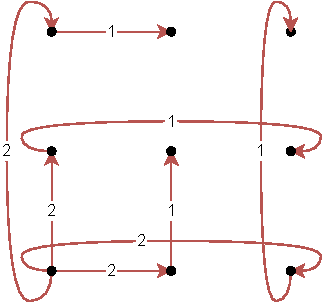
\includegraphics[width=0.6\textwidth]{q11-a}
      \end{center}
    \end{solution}

    \part Explain carefully how to use your spanning tree $T$ so as to obtain a routing algorithm in $Q_2^3$ that under the all-to-all traffic pattern results in every channel of $Q_2^3$ having the same load. 
    \begin{solution}
      To utilise our spanning tree $T$, we first show that $Q^3_2$ is node-symmetric. 
      Consider the following.
      \begin{enumerate}
        \item $\varphi_1(\overline x_1, \overline x_2) = (\overline{x_1 + 1}, \overline x_2)$; and
        \item $\varphi_2(\overline x_1, \overline x_2) = (\overline x_1, \overline{x_2+1})$.
      \end{enumerate}
      We claim that these both define automorphisms. For any $\bm x, \bm y$, it is clear that if $\varphi_1(\bm x) = \varphi_1(\bm y)$ then $\bm x = \bm y$ and similarly for $\varphi_2$; thus both define permutations. Now, let $(\bm x, \bm y)$ be a channel. Then $(\varphi_1(\bm x), \varphi_1(\bm y))$ is clearly also a channel (think about moving horizontally along the $3$-ary $2$-cube). A similar logic holds for $\varphi_2$. Now, we see by using $\varphi_1$ and $\varphi_2$, we can traverse every node on the network. Thus, $Q^3_2$ is node-symmetric. Therefore, by moving $T$ (using compositions of $\varphi_1$ and $\varphi_2$), we can obtain a routing algorithm for any source to any destination in which \emph{every channel has the same node} (this can be shown by simply studying the spanning tree, and by using the node-symmetry of $Q^3_2$).
    \end{solution}
  \end{parts}
